\section{Warum p2p?}
    Das vorausgegangen Projekt einer Verbindungskonfiguration von IoT-Geräten \linebreak \cite{aiProject} hat gezeigt, dass eine initiale p2p Verbindung aufgebaut werden muss, um eine Wi-Fi Verbindung konfigurieren zu können. In Verbindung mit einer ad-hoc Verbindung muss auch gleichzeitig eine Service Discovery betrachtet werden, um den initialen verbindungslosen Informationsaustausch über mögliche Verbindungspartner zu ermöglichen. Diese  findet aktuell ebenfalls über Wi-Fi Direct in Form von {\it DNS Service Discovery} statt. Dies hat den Vorteil, dass sich zusätzliche Daten mit einem einzigartigen Schlüssel dem Eintrag eines Service hinzufügen lassen. Eine p2p Technologie muss somit nicht zwingend verbindungslosen Beacon Signale mit Nutzdaten zur Verfügung stellen, da auch eine Hybridlösung genutzt werden kann. Das Erkennen von verfügbaren Services funktioniert bereits stabil über Wi-Fi Direct, somit wird im Weiteren lediglich der Aufbau einer p2p Verbindung thematisiert.
    
    Eine direkte Verbindung zwischen zwei Endgeräten ist nötig, wenn Daten zwischen Anwendungen ausgetauscht werden sollen und keine Verbindung über ein gemeinsames Netzwerk oder einen Server stattfinden kann oder soll. Mögliche Anwendungsfälle einer solchen p2p Verbindung sind oftmals die kabellose Nutzung von Peripheriegeräten oder der Austausch von Dateien ähnlich zu {\it Apple Air Drop}. Verbindungen zwischen Endgeräten ohne die Nutzung einer bestehenden Netzwerkinfrastruktur resultiert in einer von der genutzten Technologie abhängigen, stark reduzierten Reichweite, welche zwischen den Geräten überwunden werden kann.
    
    Das Zustandsmodell \reffig{p2p:state} eines p2p Verbindungsaufbaus lässt sich aus Sicht der beteiligten Geräte soweit vereinfachen, dass lediglich fünf von außen beobachtbare Zustände für eine erfolgreiche Nutzung der Verbindung relevant sind. Damit der Nutzer beim Verbindungsaufbau lediglich in den Prozess mit seinem Smartphone interagieren muss, sollte der p2p Verbindungsaufbau seine Zustände so vereinfacht darstellen können, um einen konsistenten Ablauf automatisiert gewährleisten zu können.
    
    Zunächst soll über den Zustand {\it INACTIVE} erkannt werden können, wenn die zu verwendende Schnittstelle ausgeschaltet ist, um sie im Ablauf des Programms einschalten zu können. Sobald der Zustand {\it IDLE} erreicht ist, kann die Schnittstelle genutzt werden, um Verbindungen über {\it ACCEPTING} zu akzeptieren oder eine neue Verbindung zu einem anderen Gerät über {\it CONNECTING} aufzubauen. Sobald ein Gerät Verbindungen annimmt und ein weiteres Gerät versucht, sich zu Diesem zu verbinden, wechseln beide Geräte im Erfolgsfall in den Zustand {\it CONNECTED} und besitzen einen gemeinsamen Kommunikationskanal. Sobald die Verbindung geschlossen wird, befinden sich beide Geräte wieder im Grundzustand {\it IDLE}. Falls eine Technologie mehr als eine parallele Verbindung erlaubt, teilt sich diese beim Akzeptieren einer neuen Verbindung auf und verbleibt weiterhin gleichzeitig im Zustand {\it ACCEPTING}.

    \begin{figure}[ht]
         \centering
	      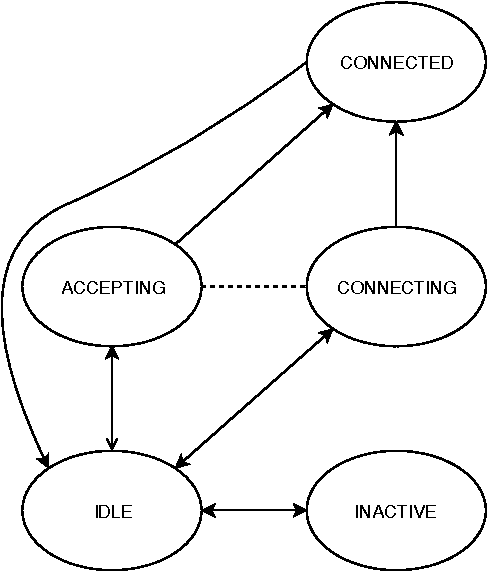
\includegraphics[width=0.5\textwidth]{p2p-State.pdf}
    	   \caption[Zustandsmodell eines p2p Verbindungsaufbaus]{Das Zustandsmodell eines p2p Verbindungsaufbaus zeigt die von außen beobachtbaren Zustände für eine erfolgreiche Nutzung einer p2p Verbindung. } \label{p2p:state}
	\end{figure}   

    Ein besonderer Nutzungspunkt für p2p Verbindungen stellen IoT-Geräte dar, da so zum einen Kommunikation ohne Konfiguration des Nutzers zwischen den IoT-Geräten stattfinden kann und eine Konfiguration der IoT-Geräte durch den Nutzer stattfinden kann ohne Peripherie an das Gerät anschließen zu müssen. Internet of Things ist ein Sammelbegriff für Gebrauchsgegenstände wie Heizungsthermostate oder Maschinen wie CNC-Fräsen, die in einer moderneren Interpretation ihrer Funktionalität über ein Netzwerk untereinander und mit Servern kommunizieren. Anwendungsgebiete können die Hausautomation, Sensornetzwerke und Betriebsüberwachung von Maschinen sein. In einem weiter gefassten Blickfeld wird unter diesem Begriff auch die Vernetzung von ganzen Städten und deren Infrastruktur untersucht \cite{ituGroup}.
    
    \subsection{Services}
    
    Im Rahmen solcher IoT-Geräte muss eine Erstkonfiguration initial vorgenommen werden, um eine Kommunikation mit anderen Geräte zu ermöglichen. Da nicht jedes Gerät einen Bildschirm oder komplexe Eingabemöglichkeiten besitzt, ist es sinnvoll, diese Einrichtung auf ein Smartphone auszulagern, wie es bereits im vorausgegangenen Projekt geschehen ist. Da die Konfiguration durch einen REST-Server angeboten wird, ist es so auch möglich, weitere Konfigurationsmöglichkeiten für Sensoren und Aktuatoren anzubieten.    
    
    - Definition eines Services
    
    - Anbieten eines Services als Client/Server-Modell
    
    \subsection{Servicestabilität (Todo: entfällt eventuell)}
    - API Versionierung
    
    - Absichern von Änderungen durch Contract-Driven-Development
    
    - Integrationstests
    \subsection{Netzwerktopologie}
		- LAN, WAN, etc.
		
		- ad hoc, Stern-basiert, Bus-basiert
